%
% File acl2014.tex
%
% Contact: koller@ling.uni-potsdam.de, yusuke@nii.ac.jp
%%
%% Based on the style files for ACL-2013, which were, in turn,
%% Based on the style files for ACL-2012, which were, in turn,
%% based on the style files for ACL-2011, which were, in turn, 
%% based on the style files for ACL-2010, which were, in turn, 
%% based on the style files for ACL-IJCNLP-2009, which were, in turn,
%% based on the style files for EACL-2009 and IJCNLP-2008...

%% Based on the style files for EACL 2006 by 
%%e.agirre@ehu.es or Sergi.Balari@uab.es
%% and that of ACL 08 by Joakim Nivre and Noah Smith

\documentclass[11pt]{article}
\usepackage{acl2014}
\usepackage{times}
\usepackage{url}
\usepackage{latexsym}
\usepackage{graphicx}
\usepackage{hyperref}
\usepackage{amsmath}
\usepackage{amssymb}
\usepackage{braket}
\usepackage{listings}


%\setlength\titlebox{5cm}

% You can expand the titlebox if you need extra space
% to show all the authors. Please do not make the titlebox
% smaller than 5cm (the original size); we will check this
% in the camera-ready version and ask you to change it back.


\title{Recursive Neural Network Part-of-Speech Tagger}

\author{Hao Liu \\
  NYU CIMS \\
  New York, NY \\
  {\tt haoliu@nyu.edu} \\\And
  Jiali Huang \\
  NYU CIMS \\
  New York, NY \\
  {\tt jiali.huang@nyu.edu} \\\And
  Robert Dionne \\
  NYU Game Center \\
  New York, NY \\
  {\tt robertsdionne@nyu.edu} \\}

\date{}

\begin{document}
\maketitle
\begin{abstract}
  TODO: Write the abstract
\end{abstract}

\section{Introduction}

For our final project, we implemented a recursive neural network part-of-speech tagger based on similar prior work by Socher, Manning and Ng (2010) for building sentence parse trees and work by Collobert and Weston (2011) for their distributed word representations. We wanted to explore natural language processing using neural networks, so we chose a small problem (part-of-speech tagging) which we already had experience with during the third homework assignment and applied these modern techniques in neural network research to the problem.

\subsection{Recursive Neural Networks}

Recursive neural networks are neural network models that allow for cyclic connections between neurons. Generally, recursive networks can have very complex structures, but for our application to part-of-speech tagging, we consider a restricted structure in which the network observes its own output on prior sentence context while consuming as input the current word in order to produce a classification label representing the current word's part of speech tag. When training the network or using the network to classify an example sentence, we temporarily unroll the recurrent network into an equivalent, feedforward multilayer perceptron with the weight matrix shared between all layers.

Our network structure is a simplification of the more general binary tree structure trained by Socher et al. (2010) which iteratively constructs a parse tree by evaluating, at the base case, the best combinations of pairs of words, and subsequently the best combinations of pairs of previous combinations. Instead, we construct a linear, degenerate tree by always pairing the current word (on the right) to the previous combination (on the left) of prior sentence context and the prior word to obtain a phrase representation. We hope that the resulting phrase representation captures both the possible parts-of-speech for the current word and distinguishing context that allows an accurate choice of the correct part-of-speech.

\subsection{Distributed Word Representations}

Underlying the entire model are distributed word representations, which we use directly from the research of Collobert and Weston (2011), downloadable from their website (\hyperlink{http://ronan.collobert.com/senna/}{ronan.collobert.com/senna}). Distributed word representations are dense vectors embedded within an $N$-dimensional vector space that differ from sparse, ``one-hot" vectors embedded within a $\left\vert\mathcal{V}\right\vert$-dimensional vector space, where $\mathcal{V}$ is the vocabulary of the language domain.

The distributed word representations are induced by training a neural network in an unsupervised manner to distinguish a word within its concrete contexts from randomly chosen replacement words within those same contexts, and then backpropagating the errors into an $N\times\left\vert\mathcal{V}\right\vert$-dimensional lookup table with randomly initialized values. The lookup table converts between the original ``one-hot" vector representation, which encodes zero information about the word aside from identity, and the superior distributed representation, which encodes a word's contextual information. Since we believe a word's context encodes information about that word's part-of-speech, we hypothesize that distributed word representations will be vital to our part-of-speech tagging model.

\section{Our Models}

We implemented a recursive neural network with the programming language Lua and the neural network library Torch7 (Collobert, 2011). Our code is available on Github at \hyperlink{http://github.com/robertsdionne/nlp}{github.com/robertsdionne/nlp}.

The first model we considered was a basic recursive neural network that combines a phrase representation $p_{i-1}$ encompassing words $w_1,w_2,\ldots,w_{i-1}$ and the word representation $w_i$ into an output phrase representation $p_i$ passed to a multilayer perceptron classifier which outputs the guessed tag.

The second model we considered was a compositional vector tagger, based upon the compositional vector grammar model by Socher, et al. (2013), in which different weight matrices are associated with different part-of-speech tags in order to generate tag-dependent phrase representations, which are then scored instead of classified. This model would perform sentence tagging by maximizing the overall score by choosing the correct tag-associated weight matrices for each word using a beam or greedy search.

The inputs to both models consist of:

\begin{center}
\begin{tabular}{ l r }
  $\mathcal{V} = \left\{w_1,w_2,\ldots,w_{\left\vert\mathcal{V}\right\vert}\right\}$ & the vocabulary \\
  $\mathcal{T} = \left\{t_1,t_2,\ldots,t_{\left\vert\mathcal{T}\right\vert}\right\}$ & the part-of-speech tags \\
  $N = 50, P = 50$ & word/phrase dimension \\
  $V\in M_{N\times\left\vert\mathcal{V}\right\vert}(\mathbb{R})$ & the word lookup table \\
  $\Ket{w_i}\in\mathcal{V}$ & the ``one-hot" vectors \\
  $V\Ket{w_i}\in\mathbb{R}^N$ & the word vectors \\
  $\Big[\bullet;\bullet\Big]$ & vector concatenation \\
\end{tabular}
\end{center}
\vspace{5mm}

\subsection{Basic Recursive Neural Network Model}

The basic recursive neural network model also has the following parameters:

\begin{center}
\begin{tabular}{ l r }
  $W_{combine}\in M_{P\times(P+N)}(\mathbb{R})$ & matrix for combining \\
  $b_{combine}\in \mathbb{R}^P$ & bias for combining \\
  $W_{classify}\in M_{\left\vert\mathcal{T}\right\vert\times P}(\mathbb{R})$ & matrix for tagging \\
  $b_{classify}\in \mathbb{R}^{\left\vert\mathcal{T}\right\vert}$ & bias for tagging \\
\end{tabular}
\end{center}

\vspace{5mm}
We began by training our model on the Penn Treebank sentences from assignment three, available at \hyperlink{http://www.cs.nyu.edu/petrov/restricted/data3.zip}{www.cs.nyu.edu/petrov/restricted/data3.zip}.

To train the model, we first initialize $W_{combine}$, $b_{combine}$, $W_{classify}$ and $b_{classify}$ with small, uniformly distributed random values. We will discuss how to choose the range for these values in section \textbf{3.2.1 Weight Initialization} below. Then we perform a classification step in which we convert each word into its distributed word representation, pass each of these representations through the unrolled recursive neural network's inputs, and feed the values forward to the classification layers corresponding to each tag output.

For instance, given the sentence $(w_{i_1},w_{i_2},\ldots,w_{i_K})$ of length $K$, we first calculate the word representations $V\Ket{w_{i_1}},\ldots,V\Ket{w_{i_K}}$, then we calculate each phrase representation $p_j$ from the previous phrase representation $p_{j-1}$ and the current word representation $V\Ket{w_{i_j}}$ by concatenating the two representation vectors, multiplying by $W_{combine}$ and adding $b_{combine}$ before applying the $tanh(\cdot)$ function:

$p_j = tanh(W_{combine}\Big[p_{j-1};V\Ket{w_{i_j}}\Big] + b_{combine})$

Subsequently, each $p_j$ is passed along to the classifier, which applies the operation:

$t_{i_j} = softmax(W_{classify}p_j + b_{classify})$

to obtain the predicted tag $t_{i_j}$ for $w_{i_j}$.

Finally, we perform backpropagation through time, described in section \textbf{3.1} below, to update the weight matrices and bias vectors. Performing a backpropagation after classifying each sentence in the dataset performs stochastic gradient descent in minibatches (where we consider one sentence to be a minibatch of tags and words) to update the weight matrices to more accurately predict the golden tags.

\subsection{Compositional Vector Tagger Model}

The second model we considered uses weight matrices that depend upon the golden tags of the training sentences. The parameters are as follows:

\begin{center}
\begin{tabular}{ l r }
  $W_{combine,t}\in M_{P\times(P+N)}(\mathbb{R})$ & matrix for tag $t$ \\
  $b_{combine,t}\in \mathbb{R}^P$ & bias for tag $t$ \\
  $W_{score}\in M_{1\times P}(\mathbb{R})$ & matrix for scoring \\
  $b_{score}\in \mathbb{R}$ & bias for scoring \\
\end{tabular}
\end{center}

\vspace{5mm}
The training and classification procedures differ from the basic model. First, in unrolling the recurrent neural network, each recurrent layer adopts the weight matrix associated with the golden tag of the word in that position. For instance, if $w_{i_3}$ had tag $t_{i_3} = \text{NN}$ then the third recurrent layer would adopt the weight matrix $W_{combine,\text{NN}}$. Each recurrent layer adopts the appropriate weight matrix before generating the phrase representations $p_j$. We then apply backpropagation to maximize the score for the representations provided by the golden tag weight matrices by updating those matrices and the score matrix.

Raw classification on unlabeled examples now requires a search procedure. The brute-force procedure to tag a sentence of length $K$ would be to search through all $K^{\left\vert\mathcal{T}\right\vert}$ sequences of tag weight matrices and return the sequence that attains the highest overall score based on the score matrix. As our tag set has size $\left\vert\mathcal{T}\right\vert=48$, this search is intractable for realistic sentences, so a greedy or beam search would need to be used instead.

As the complexity of the compositional vector tagger model is significantly higher than the basic recurrent neural network model, we were unable to properly train the model and implement a satisfactory search procedure within the remaining time of the assignment, so we have omitted analysis of the results of this model.

\subsection{Future Models}

TODO: Describe future models.

\section{Experiments}

Our experiments consisted of training the recursive network on training sentences drawn from the Penn Treebank data of assignment three, as we described above. We frequently trained on 100, 1000, 10,000 or 39,815 (all) of the training sentences in exploring the performance of the recursive neural network for part-of-speech tagging. Training on the entire data set for 25 iterations, or on 10,000 training sentences for 100 iterations, each took about 4 hours on a 2012 Macbook Pro Retina with a 2.6 GHz Intel Core i7 CPU and 8 GB of RAM.

To evaluate the network, we used a basic metric which counts the ratio of the number of correctly tagged words out of the total number of words within the validation or test set (1700 in-domain validation sentences, 1016 out-of-domain validation sentences and 1015 out-of-domain test sentences). We also count the ratio of correctly tagged unknown words, where a word is defined to be unknown if it was not encountered during the training set; however, note that it may be present within $\mathcal{V}$, the vocabulary associated with the distributed representation lookup table. If the word is unknown to the distributed representation lookup table, the model falls back upon the distributed representation for the special token ``UNKNOWN."

\subsection{Backpropagation Through Time}

TODO: Describe back propagation through time.

\subsection{Training Tricks}

Training neural networks can be tricky since the backpropagation algorithm relies upon a learning rate parameter as well as initial weight and bias values. The learning rate should not be too large, otherwise the gradient descent will skip over local or global minima. However, it should also not be too small, otherwise training may take too long. It perhaps should vary over the course of training and decrease in order to better fine tune the fit to the minima. However, it's not obvious exactly which set of choices will be best.

We researched existing techniques to choose initial weights and biases, and to better update the weights based on adaptive learning rates, as described in the next subsections.

\subsubsection{Weight Initialization}

Early on, we randomly initialized our weight matrices and biases using Torch7's uniform tensor function,
\begin{lstlisting}
torch.rand(P, P+N)
torch.rand(P)
\end{lstlisting}
which draws from $\mathcal{U}[0, 1)$ however, we discovered guidelines for weight initialization from \hyperlink{http://deeplearning.net/tutorial/mlp.html\#mlp}{deeplearning.net/tutorial/mlp.html\#mlp}, borrowed from Glorot and Bengio (2010), and decided to explore how they impacted our training convergence.

Glorot and Bengio (2010) analyzed how initial values for weights influenced the early learning of neural networks, specifically those that use $tanh(\cdot)$ or $sigmoid(\cdot)$ and discovered optimal early learning rates with weights drawn from
\begin{itemize}
\item $\mathcal{U}\Big[-\sqrt{\frac{6}{fan_{in}+fan_{out}}},\sqrt{\frac{6}{fan_{in}+fan_{out}}}\Big)$ for $tanh$ layers
\item $\mathcal{U}\Big[-4\sqrt{\frac{6}{fan_{in}+fan_{out}}},4\sqrt{\frac{6}{fan_{in}+fan_{out}}}\Big)$ for $sigmoid$ layers
\end{itemize}
where $fan_{in}$ is the number of inputs to the layer and $fan_{out}$ is the number of outputs.

After adopting these new ranges, and initializing our biases to start at zero, our attainable accuracies dramatically increased from the values we presented in class in our slides, from about $60\%$ to about $80\%$.

\subsubsection{AdaGrad}

TODO: Describe AdaGrad.

\subsection{Analysis}

TODO: Describe analysis.

\subsubsection{Training Progress Diagram}

TODO: Describe training progress diagrams.

\subsubsection{Comparison to Other Models}

TODO: Compare to baseline.

TODO: Compare to HMM.

\subsubsection{Error Analysis}

\paragraph{Confusion matrices} 
We plot the confusion matrix (Figure \ref{Conf_fig}) for the basic RNN model and find that:
\begin{enumerate}
\item The \textbf{most serious confusion is between NNP and NN}. This makes sense because of the fact that the embeddings we are using make no distinction between capitalized and non-capitalized words;
\item  Another strange confusion is from quotes, which was also met in common HMM models. This may come from the overwhelming sequential information;
\item Other confusions look normal, and also occur in HMM models, like JJ and NN.
\end{enumerate}
\begin{figure}
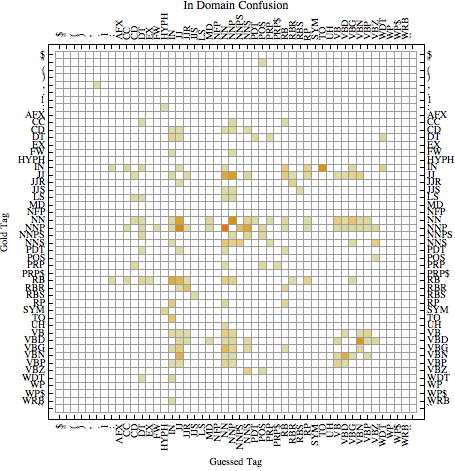
\includegraphics[scale=0.5]{indomain_conf.png} 
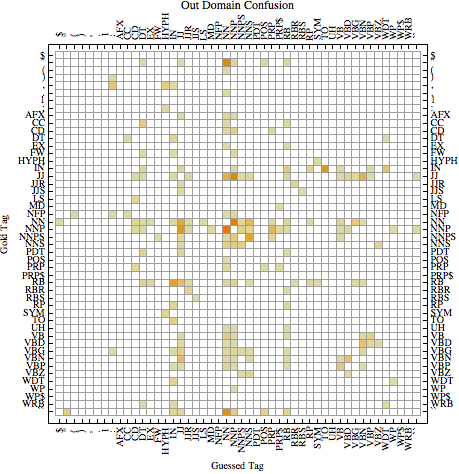
\includegraphics[scale=0.5]{outdomain_conf.png} 
\caption{Confusion matrices for basic RNN}\label{Conf_fig}
\end{figure}



\paragraph{Position of wrong tags } 
We plot the histogram (Figure \ref{Pos_fig}) of relative position (absolute position in sentence divided by sentence length in (0, 1]). 
\begin{itemize}
\item \textbf{In-domain} (left figure): The relative position is almost uniformly distributed.
\item \textbf{Out-of-domain} (right figure): The number of wrong tags is generally increasing with relative position. And from the different scale of this histogram, we find there is a big drop around 0.5 (middle of sentence). This may come from the sequential similarity between in-domain and out-of-domain. This may also come from the limitation of sequential information passing. So a bi-directional RNN may help.
\end{itemize}
\begin{figure}
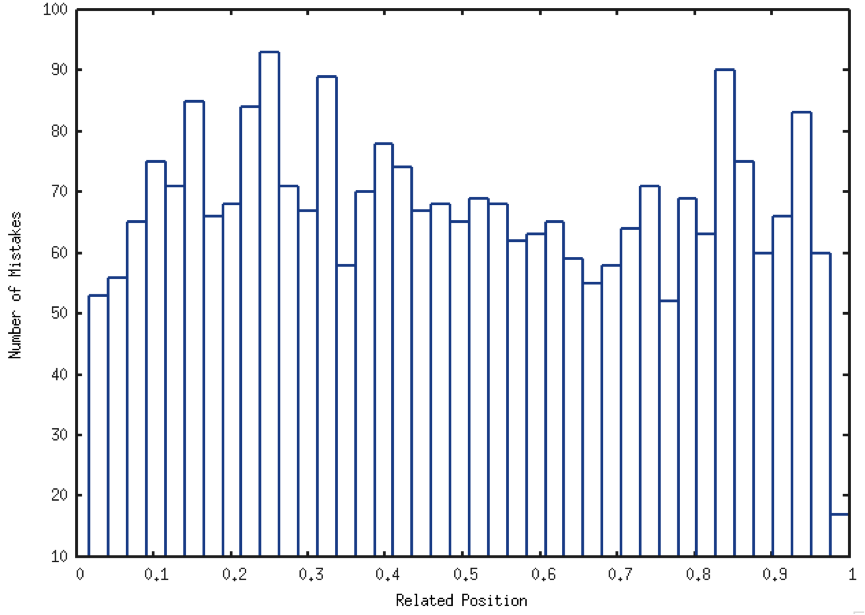
\includegraphics[scale=0.25]{indomain_pos.png} 
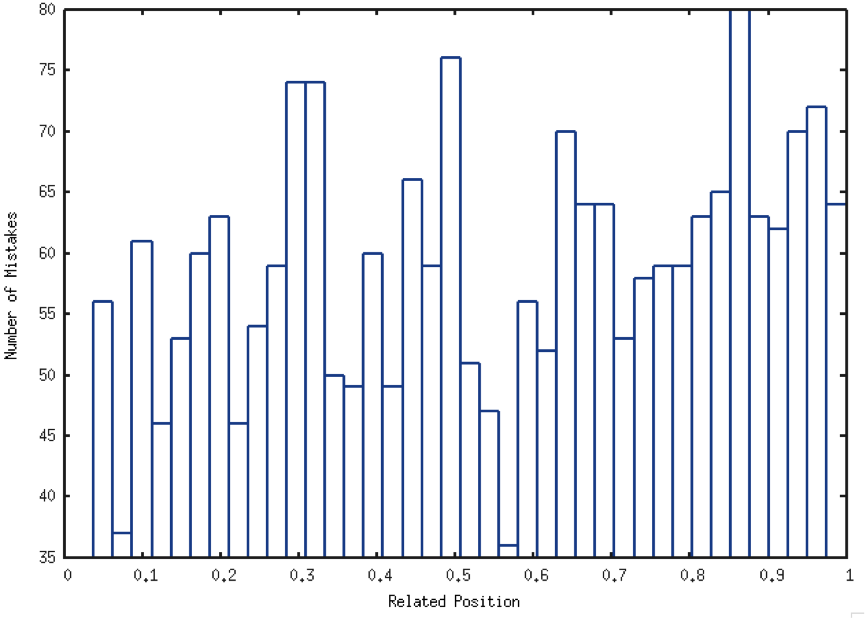
\includegraphics[scale=0.25]{outdomain_pos.png} 
\caption{Histogram of related position of wrong tags, left is in domain, right is out of domain}\label{Pos_fig}
\end{figure}

\paragraph{Not just a maximum likelihood model}
In the beginning, we worried about whether this RNN model can pass and use the sequential information correctly. Perhaps it just learns a maximum likelihood (most frequent) predictor for each word or even each group of words. So we did some experiments to verify the contribution of sequential information to the RNN results.

\begin{itemize}
\item \textbf{Same word test}:  We chose some words with more than one common tag and saw whether our model predicted those tags correctly. We tested on `to' (possible tags are TO and IN) and `work' (common possible tags are NN, VB and VBP). Our RNN predicts `to' with 0.80 in-domain and 0.77 out-of-domain accuracy, covering TO and IN. The RNN predicts `work' with 0.88 in-domain and 0.83 out-of-domain accuracy, covering NN, VB and VBP.
\item \textbf{Disconnected core module test}: We disconnected the sequential information passing by ignoring the input embeddings from lower layers, and backward gradient from upper layers. So although it's still an RNN, there is actually no information passed between layers. We trained this non-sequential RNN and the original RNN with 100 sentences and 100 iterations, same random seed and training parameters. The Figure \ref{Noseq_fig} shows the out-of-domain accuracy of two models by the number of iterations, which can be also seen from Figure \ref{Leftsize_fig}. The difference is not small. So we think the sequential information was passed and used at least partially correctly.
\end{itemize}
\begin{figure}
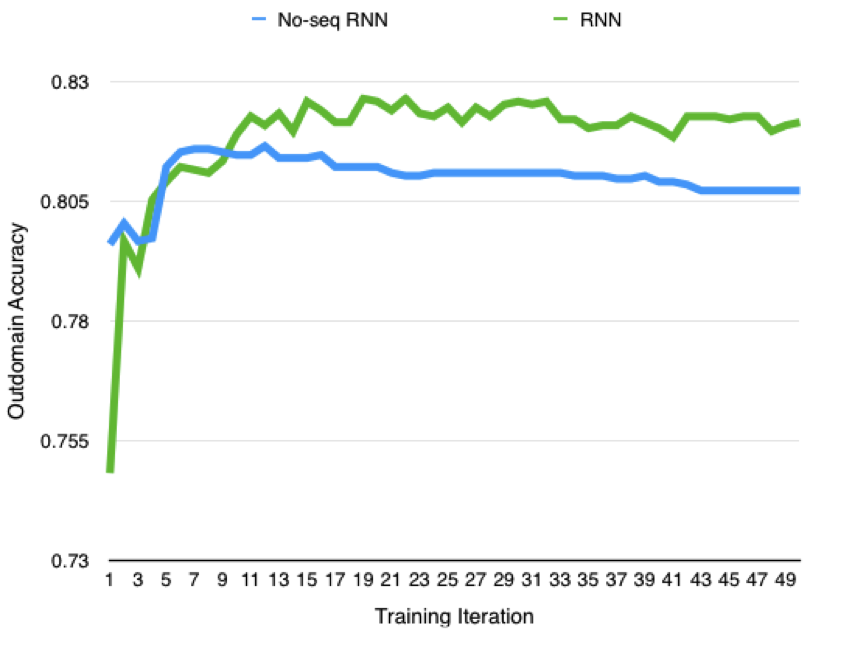
\includegraphics[scale=0.5]{outdomain_noseq.png}
\caption{Comparison of non-sequential RNN and original RNN for disconnected core module test}\label{Noseq_fig}
\end{figure}

\paragraph{Different embedding size of state}
The size of state embeddings (left side of each RNN layer) is another hyper-parameter to set up. And it is important because it may determine the importance of previous sequential information compared to the current word embedding. Figure \ref{Leftsize_fig} shows the the out-of-domain accuracy of two models by the number of iterations. And it looks like 20 is around the optimal size for state embeddings.
\begin{figure}
	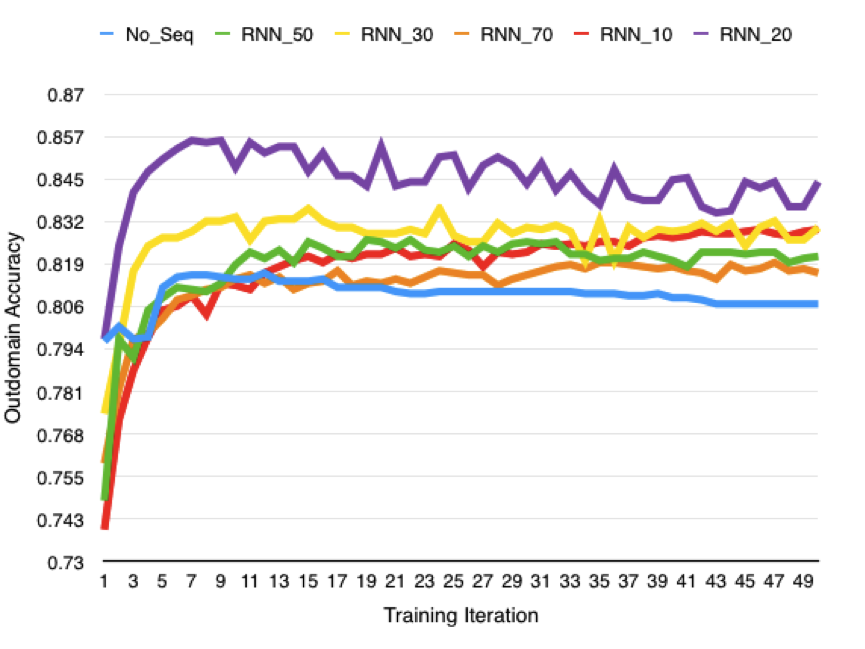
\includegraphics[scale=0.5]{outdomain_leftsize.png}
	\caption{Out-of-domain accuracy comparison of different state embedding size} \label{Leftsize_fig}
\end{figure}

TODO: Compare with and without updating word representations.


TODO: Specific error examples and hypotheses.





\section{Conclusion}

\section{Academic Honesty Pledge}

Honor Pledge

We pledge our honor that all the work described in this report is solely ours and
that we have given credit to all third party resources that we have used.

% include your own bib file like this:
%\bibliographystyle{acl}
%\bibliography{acl2014}

\begin{thebibliography}{}

\bibitem[\protect\citename{Collobert and Weston}2011]{Collobert:11}
Ronan~Collobert, Jason~Weston, LŽon~Bottou, Michael~Karlen, Koray~Kavukcuoglu and Pavel~Kuksa.
\newblock 2011.
\newblock Natural Language Processing (Almost) from Scratch.
\newblock {\em Journal of Machine Learning Research 12},  (2011) 2461-2505.
\newblock The MIT Press, Cambridge, MA.

\bibitem[\protect\citename{Collobert, Kavukcuoglu and Farabet}2011]{Collobert:11}
Ronan~Collobert, Koray~Kavukcuoglu and ClŽment~Farabet.
\newblock 2011.
\newblock Torch7: A matlab-like environment for machine learning.
\newblock {\em BigLearn, NIPS Workshop}.

\bibitem[\protect\citename{Glorot and Bengio}2010]{Glorot:10}
Xavier~Glorot and Yoshua~Bengio.
\newblock 2010.
\newblock Understanding the difficulty of training deep feedforward neural networks.
\newblock {\em International Conference on Artificial Intelligence and Statistics}.

\bibitem[\protect\citename{Socher, Bauer, Manning and Ng}2013]{Socher:13}
Richard~Socher, John~Bauer, Christopher~D. Manning and Andrew~Ng.
\newblock 2013.
\newblock Parsing with Compositional Vector Grammars.
\newblock {\em In Proceedings of the ACL conference}.

\bibitem[\protect\citename{Socher, Manning and Ng}2010]{Socher:10}
Richard~Socher, Christopher~D. Manning and Andrew~Ng.
\newblock 2010.
\newblock Learning Continuous Phrase Representations and
Syntactic Parsing with Recursive Neural Networks.
\newblock {\em Proceedings of the NIPS-2010 Deep Learning and Unsupervised Feature Learning Workshop}.

\end{thebibliography}

\end{document}
